
%% 
%% Copyright 2007-2019 Elsevier Ltd
%% 
%% This file is part of the 'Elsarticle Bundle'.
%% ---------------------------------------------
%% 
%% It may be distributed under the conditions of the LaTeX Project Public
%% License, either version 1.2 of this license or (at your option) any
%% later version.  The latest version of this license is in
%%    http://www.latex-project.org/lppl.txt
%% and version 1.2 or later is part of all distributions of LaTeX
%% version 1999/12/01 or later.
%% 
%% The list of all files belonging to the 'Elsarticle Bundle' is
%% given in the file `manifest.txt'.
%% 
%% Template article for Elsevier's document class `elsarticle'
%% with harvard style bibliographic references

% \documentclass[preprint,12pt,authoryear]{elsarticle}
% \usepackage{graphicx}

% \usepackage{epstopdf}
% \epstopdfDeclareGraphicsRule{.pdf}{png}{.png}{convert #1 \OutputFile}
% \DeclareGraphicsExtensions{.png,.pdf}

%% Use the option review to obtain double line spacing
%% \documentclass[authoryear,preprint,review,12pt]{elsarticle}

%% Use the options 1p,twocolumn; 3p; 3p,twocolumn; 5p; or 5p,twocolumn
%% for a journal layout:
%% \documentclass[final,1p,times,authoryear]{elsarticle}
\documentclass[final,1p,times,twocolumn,authoryear]{elsarticle}
%% \documentclass[final,3p,times,authoryear]{elsarticle}
%% \documentclass[final,3p,times,twocolumn,authoryear]{elsarticle}
%% \documentclass[final,5p,times,authoryear]{elsarticle}
%% \documentclass[final,5p,times,twocolumn,authoryear]{elsarticle}

%% For including figures, graphicx.sty has been loaded in
%% elsarticle.cls. If you prefer to use the old commands
%% please give \usepackage{epsfig}

%% The amssymb package provides various useful mathematical symbols
\usepackage{amssymb}
%% The amsthm package provides extended theorem environments
%% \usepackage{amsthm}

\usepackage{lineno}

\usepackage{longtable}
\usepackage{hyperref}
\usepackage{natbib}

%% The lineno packages adds line numbers. Start line numbering with
%% \begin{linenumbers}, end it with \end{linenumbers}. Or switch it on
%% for the whole article with \linenumbers.
%% \usepackage{lineno}

\journal{Patterns}

\newcommand{\cvm}[1]{\protect{\texttt{{#1}}}}
\newcommand{\om}{O\&M}

\begin{document}

\begin{frontmatter}

%% Title, authors and addresses

%% use the tnoteref command within \title for footnotes;
%% use the tnotetext command for theassociated footnote;
%% use the fnref command within \author or \address for footnotes;
%% use the fntext command for theassociated footnote;
%% use the corref command within \author for corresponding author footnotes;
%% use the cortext command for theassociated footnote;
%% use the ead command for the email address,
%% and the form \ead[url] for the home page:
%% \title{Title\tnoteref{label1}}
%% \tnotetext[label1]{}
%% \author{Name\corref{cor1}\fnref{label2}}
%% \ead{email address}
%% \ead[url]{home page}
%% \fntext[label2]{}
%% \cortext[cor1]{}
%% \address{Address\fnref{label3}}
%% \fntext[label3]{}

\title{Exploiting and Extending Vocabularies for Faceted Browse in Earth System Science}


%% use optional labels to link authors explicitly to addresses:
%% \author[label1,label2]{}
%% \address[label1]{}
%% \address[label2]{}

\author[1]{Ruth E. Petrie}
\author[2,3]{Bryan Lawrence}
\author[1]{Martin Juckes}
\author[1,4]{Victoria Bennett}
\author[4]{Philip Kershaw}
\author[1]{Ag Stephens}
\author[4]{Alison Waterfall}
\author[5]{Antony Wilson}

\address[1]{National Centre for Atmospheric Science, CEDA, Science and Technology Facilities Council, UK}
\address[2]{National Centre for Atmospheric Science, Department of Meteorology, University of Reading, UK}
\address[3]{Department of Computer Science, University of Reading, UK}
\address[4]{National Centre for Earth Observation, CEDA, Science and Technology Facilities Council, UK}
\address[5]{Scientific Computing Department, Science and Technology Facilities Council, UK}


\begin{abstract}

The earth system grid federation (ESGF) deployed a faceted browsing system for finding data within a large (petascale) globally distributed climate data archive. This system relied on a ``Data Reference Syntax'' which was designed initially for providing meaningful navigable identifiers for data from the fifth climate model intercomparison project (CMIP5). In this paper we provide additional context and expand on the need for such systems, discuss the inherent dependencies on controlled vocabularies, and show how the DRS concept has been extended to provide support for additional projects (CORDEX, CLIPC, CMIP6). We discuss the nature of search and browse and the impact of linked data concepts on successful data discovery. We also discuss the wider applicability in environmental science of faceted browse coupled with meaningful data identifiers.

\end{abstract}

%%Graphical abstract
% \begin{graphicalabstract}
%  \includegraphics{grabs}
% \end{graphicalabstract}

% %%Research highlights
% \begin{highlights}
% \item Research highlight 1
% \item Research highlight 2
% \end{highlights}

\begin{keyword}
Earth System Science \sep
Data \sep 
Metadata \sep
Data Reference Syntax \sep 
Faceted searching

%% keywords here, in the form: keyword \sep keyword

%% PACS codes here, in the form: \PACS code \sep code

%% MSC codes here, in the form: \MSC code \sep code
%% or \MSC[2008] code \sep code (2000 is the default)

\end{keyword}

\end{frontmatter}

%% \linenumbers

%% main text

\section{Introduction}

Earth System Science (ESS) has always had difficulties associated with both the number and volume of data products. 
These difficulties arise because both earth observation and numerical simulation involve continually increasing data production driven by underlying trends in computing, always at the edge of what is possible, and so managing and manipulating such data at scale has always required heroic effort.
For example the European Space Agency Sentinel satellites \citep{BerEA12} are currently (2018) approaching 15 TB/day \citep[5PB/year ---][]{Sentinel2019} and next iteration (phase 6) of Coupled Model Intercomparison Project (CMIP6) is anticipated to produce around 10-20 PB of data in the 2019-2020 timeframe.
  
 One of the many challenges with this data is facilitating the discovery and use of climate data records. 
 Climate data comes from a variety of sources such as modelling (including global, regional and seasonal modelling), earth observation (e.g. from satellites, in-situ observations, radiosondes etc.), reanalysis (a combination of both model and observational data0 and climate impact indicators (derived products). 
 All these different climate data products are produced within different parts of the ESS community and it is common for the different communities to have different data conventions (such as file formats) and standards. 
 Nonetheless, these heterogeneous data need to be processed automatically, a problem which grows larger with increasing volume and heterogeneity. 
Such automated processing requires the use of data description and organisation methodologies which are well defined and structured, which support discovery via multiple methods and entry points, and can be applied consistently across the ESS community.

In this paper we discuss two key methodologies: controlled vocabularies and structured syntaxes to support faceted browse, and their application in both the Climate Information Platform for Copernicus (CLIPC) and the Earth System Grid Federation. 

Controlled vocabularies are sets of terms and definitions which have some managed process for change and maintenance which attempts to maximise accuracy, minimise ambiguity and repetition, and support incremental updates.
They are typically managed in computer systems which provide both human and machine readable interfaces (e.g. the NERC vocabulary service available at \href{https://www.bodc.ac.uk/resources/products/web\_services/vocab/}
{https://www.bodc.ac.uk/resources/products/web\_services/vocab/}, 
 \citealt{Latham2009, Leadbetter2012}). 

Faceted Browse is a particular form of data navigation which will be familiar to many people from application in internet shopping where a set of search results can be progressively refined by a set of pre-defined characteristics of the products (e.g. when shopping for fridges, refining by dimensions, manufacturer, energy rating etc).  An important characteristic of faceted browse is that it is not hierarchical (e.g. for the fridge purchase example, one could start with manufacturer and refine, or start with energy rating and refine, etc).

\textit{TODO: Ruth: Add paragraph on paper layout here, based on the following original text and the eventual structure of the paper}
In this paper we are interested in how the known technologies of faceted search is applied and utilised in the ESS and how this could be applied to other scientific disciplines.

In order to achieve this two things are required. Firstly, a framework of both hardware and software infrastructure that supports for faceted searching is required and secondly a well defined set of controlled vocabularies that are widely adopted by the community.  

It is essential that both the data and metadata are easily accessible to all users. In the context of “big data” this means not only that users are able to discover the information that they need but also that they are able to work with the data within their information handling systems. This consists of two key aspects: (1) Technical and domain specific terms must have accessible definitions and (2) Such definitions must be provided in a form that other peoples' software can work with. 


The aims of this paper are to describe the issues around data discovery through faceted search in the climate modelling community through a demonstration of how the research project the Climate Information Platform for Copernicus (CLIPC) ?REF? utilised and extended the existing infrastructure to provide a single point of access to a variety of heterogeneous data. 


\subsection{Data Discovery}

The notion of data discovery is understood by different communities differently, and even within one community the concept can mean different things depending on application. 
For example, for some earth observation users, discovering a dataset would mean finding the set of all images from all sensors which are relevant for their location at a specific time, and for others, it might be to discover the set of all images from a particular sensor.
How this can be supported is a function of the available metadata, the way the data is organised, and the software which provides the discovery service. In particular, the success or failure of such discovery is often dependent on how the data publisher has organised data into datasets, what navigation facilities are provided to find datasets, and whether-or-not and how, datasets can be subsetted.

There are two key steps involved in finding data which can be characterised as teleporting and orienteering \citep{Teevan2004}: the former involves ``jumping'' to the neighbourhood where the right data can be found, and the latter, to the process of navigating around to find exactly what is wanted. 
These two steps need to be supported by data metadata. 
In practice there are several sorts of relevant metadata, particularly where data is kept in files on a disk or tape system as is often the case for high volume ESS data: metadata held in the files, metadata which appears in the physical layout of the files (e.g. directory names on a file system) and metadata held in databases or web-pages. 
Whatever their source and location, they can be characterised using the taxonomy introduced in \cite{LawEA09}: ``A for archive'' data is necessary to navigate (orienteer) around a file system, potentially utilising information held in the files and the filepaths, ``B for Browse'' metadata is also used for navigation, but also to discriminate between similar datasets (e.g. two model simulations of the same phenomenon). 
``C-Character'' holds information about actual or perceived quality, and ``D-Discovery'' provides the equivalent of dataset catalogue records, providing the information necessary for teleporting (to find a point from where one can orienteer).

If the datasets are not organised with sufficient granularity, or datasets structures differ, then many discovery use cases cannot exploit orienteering, either because the datasets are too large (one does not get close enough with teleporting for orienteering to work), or because the method of orienteering is too different between datasets. 
When the information system and/or data are predominantly hierarchical (organised in simple tree structures) this problem is exacerbated. While teleporting can arrive at some point ``in the tree'', it becomes difficult to find similar parts of multiple trees via orienteering, unless the trees have similar structures.
When the datasets have too much granularity, there are too many potential teleporting targets and so the metadata system needs to compensate so that it can produce aggregated views that can be unfolded into the constituent parts as orienteering proceeds.
The obvious difficulty with aggregation is that there may be many different ways to do the aggregation.

Faceted browse with aggregation provides a sophisticated method of dealing with some of these issues, but only if it is underpinned by controlled vocabularies which ensure that different datasets can be viewed and/or aggregated using commonly understood terms. 
Datasets then need to be tagged with the correct combination of terms, and the information system (hardware and software) need to deliver the requisite functionality. 
Here we concentrate on the vocabularies and dataset granularities needed to deliver \dots

%TODO: Ruth completion
\textit{TODO: Ruth: COMPLETE}.
 
\section{Data Reference Syntax}
\subsection{History}
\label{s:history}

At the advent of the fifth climate model intercomparison project, CMIP5, it was apparent that the community was going to be faced with at least a petabyte of data organised into at least a million files. 
Data was being produced by multiple organisations, using different software systems (models) according to the needs of a variety of experiments, and consisting of hundreds of different output variables being produced by simulations of ocean, atmosphere, land surface, etc.  
It was going to be housed in distributed federation of data nodes, and users were going to be expected to find and download only the data of interest to them.

Experience from the earlier CMIP exercises had led to the knowledge that structured metadata was crucial, so the notion of quality A-metadata was already present, and it was known that mixing different variables within files could be problematic (greater chance for errors in any given file, more likelihood that users downloading files would be downloading data they didn't need). 
However, it was also known that different groups liked to organise their data differently. 
The solution which arose was the ``Data Reference Syntax" (DRS) introduced in \cite{TayEA12}, which provided a human and machine readable structured identifier for what became known as ``atomic datasets'' (nearly indivisible granules of data). 
The DRS identifier utilised controlled vocabularies to provide CMIP5 both landing points for teleporting, and a nomenclature for a host of important routes to aggregating the atomic datasets.  
It was also completely agnostic about file organisation (it is often necessary to remind people that the D does not stand for "Directory") allowing different groups to organise their data as they preferred.

The set of vocabularies which were chosen to construct a CMIP5 DRS identifier are listed in table \ref{cmip5-drs}.
An individual identifier is constructed by using vocabulary members constructed by concatenating them all in specific sequence separated by a dot: 
\begin{quote}
\small\texttt{
\textless{}project\textgreater{}.\textless{}product\textgreater{}.\textless{}institute\textgreater{}.\textless{}model\textgreater{}.\textless{}experiment\textgreater{}.\textless{}time\_frequency\textgreater{}.\newline
\textless{}realm\textgreater{}.\textless{}cmor\_table\textgreater{}.\textless{}ensemble\textgreater{}.\textless{}version\textgreater{}}
\end{quote}
for example
\begin{quote}
 \small\texttt{CMIP5.MPI-M.MPI-ESM-LR.amip.mon.land.Lmon.r5i1p1.v20120529}
 \end{quote}


\begin{table}[ht!]
\label{tab:cmip5}
\begin{tabular}{|p{3cm}|p{9.5cm}|}
\hline
\textbf{Facet}  & \textbf{Definition}  \\ \hline
project         & Fixed as CMIP5\\ \hline
product         & The type of output produced by the model. \\ \hline
institute       & The climate modelling centre(s) or University responsible for the model. \\ \hline
model           & The specific name of the climate model used.  \\ \hline
experiment      & The valid CMIP5 experiment short identifier.  \\ \hline
time frequency  & The temporal frequency of the output data, e.g. ``mon" for monthly data.  \\ \hline
realm           & The earth system realm of the data, e.g. ``atmos" for the atmosphere. \\ \hline
CMOR table      & A lookup table that relates the frequency of a variable and its realm.    \\ \hline
ensemble member & The specific ensemble member of the model run of the form r\textless{}L\textgreater{}i\textless{}M\textgreater{}p\textless{}N\textgreater where, L M and N are integers and r is for realisation; i for initialisation and p is for physics. \\ \hline
version         & This is an ESGF version to uniquely identify the dataset and version control the data, it is given the form vYYYYMMDD. \\
\hline

\end{tabular}
\caption{Facet definitions for CMIP5 \label{cmip5-drs}}
\end{table}

%TODO: This is not a complete list of CMIP5 identifiers, should we say something about the subset identifiers?

\subsection{The use of the DRS to support faceted browse in the ESGF}

The CMIP5 data were distributed by the Earth System Grid Federation (ESGF), an international collaboration built on a shared experience developing and deploying software infrastructure over the last two decades.
 It was initially designed to handle the CMIP5 project alone \citep{WilEA11_esgf}, but has since grown to encompass a number of other projects, all deploying variants of the original DRS.  
 It now hosts in excess of 20 PB, and has been integral to recent assessments made by the Intergovernmental Panel on Climate Change (IPCC).

The ESGF is a global system with nodes distributed around the world and all continents represented.
Nodes interoperate with each other using a peer-to-peer paradigm, and provide the same set of standardised data search and access protocols.
Some nodes host data replicated from other nodes, but most simply provide local data for remote discovery and download. 

The ESGF supports multiple projects, and the ESGF data discovery service relies heavily on the DRS concept, even for non-CMIP projects.  The DRS identifier is the unique identifier which allows the system to know which datasets are replicated between nodes, and provides facets that both supports faceted browse in the discovery user interface and allows downstream applications to construct faceted search interfaces to ESGF data.  An example of the faceted browse interface appears in figure \ref{fig:search-esgf-cmip5}.

\begin{figure}[ht!] 
\centering
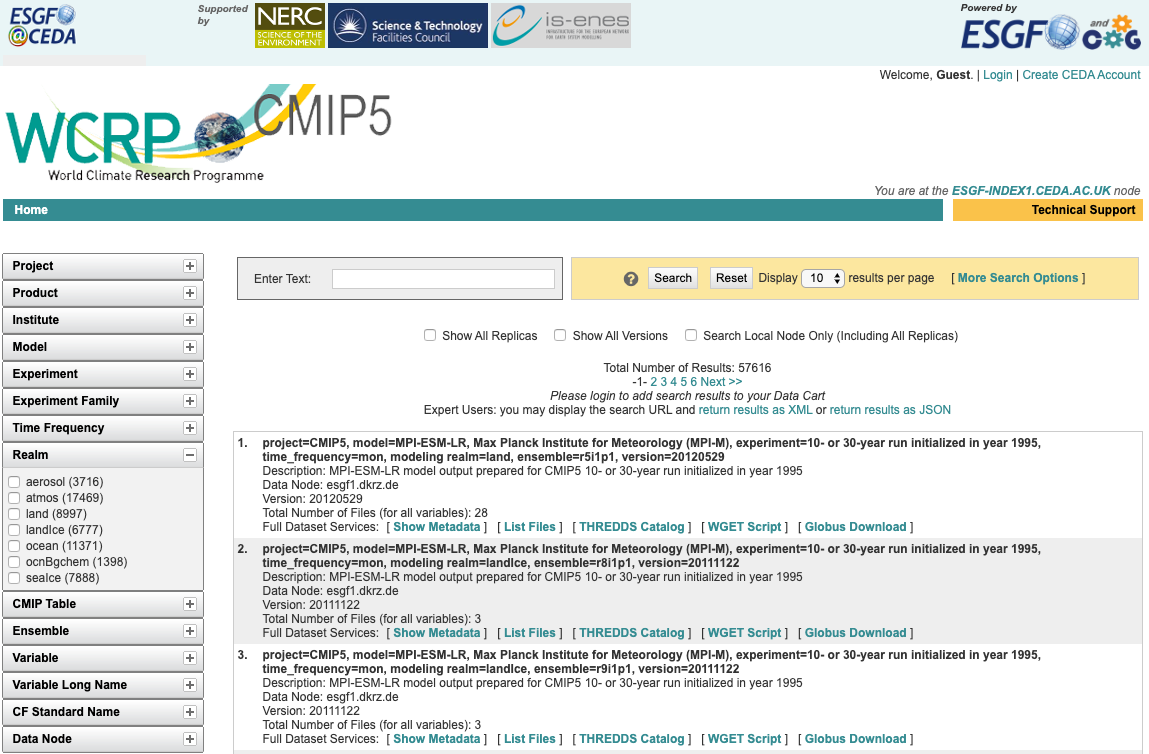
\includegraphics[scale=0.32]{images/esgf_cmip5.png}
\caption{Screenshot of the Earth System Grid Federation (ESGF) CMIP5 faceted search interface. This example shows a case where no facets have been select so all results are returned. The CMIP5 \texttt{realm} facet is  expanded on the left hand side showing the potential to select datasets from the seven different options in the CMIP5 realm vocabulary.\label{fig:search-esgf-cmip5} }
\end{figure}


\subsection{Underlying DRS principles for the ESGF}

The experience in ESGF showed that the DRS concept of conflating an identifier with a compound set of facets was very powerful, providing both machines and humans real utility. 
However, this utility does not arise from chance, and it depends on the right set of facets, which in turn depend on how they are structured.
Facet terms should either be terms from a controlled vocabularies or be of a flexible structured form (e.g. sub-ranges within an axis, such as periods within a date range).

A controlled vocabulary (CV) is simply a list of terms with an associated precise definition that must be replicated in a precise form (including spelling, case and other characters). 
Controlled vocabularies are widely used to organise and annotate large volumes of data, and are often used in file naming conventions, or to populate internal file metadata.  
For use as an identifier and as facets they need to be un-ambiguous, fully partition the space of possible terms, and be distinct (no dataset may fall outside the domain of the vocabulary, or be capable of annotation by more than one term in each vocabulary).
For example, the CMIP5 facet \cvm{Realm} spans the full set of high level modelling domains expected within an earth system model, and can only take one of the permitted values: \cvm{atmos}, \cvm{ocean}, \cvm{land}, \cvm{landIce}, \cvm{seaIce}, \cvm{aerosol}, \cvm{atmosChem}, and \cvm{ocnBgchem} (where the latter covers ``ocean bio-geochemistry'' and the rest should be self evident). 
Ensuring that these requirements are met is why they need ``control'' --- it must be difficult to inadvertently break these criteria, yet also allow new terms to be added as would be necessary if either the domain is expanded, or the facets need sub-division.

Facets which encompass flexible structures similarly need to span the range with no overlapping, but they too need to be controlled to an extent to ensure the facets are meaningful across data providers.  

As an example, the CMIP5 facet ``Ensemble member'' must unambiguously identify all possible ensemble members within an ensemble (a set of simulations which vary somehow across a particular experimental configuration). However, while the extent of the domain of such ensemble members may not be known except by the data provider (and hence is not encoded), the structure of the possible domain is prescribed, in this case to a triplet of the form  \cvm{r\textless{}L\textgreater{}}i\textless{}N\textgreater{}p\textless{}M\textgreater{} where \cvm{L,N} and \cvm{M} are integers and \cvm{r, i} and \cvm{p} indicate realisation, initialisation, and physics axes respectively, so that ensemble members can be identified in the space of all simulations carried out by a particular provider along those axes. So \cvm{r3i2p1} indicates the third realisation of the second kind of initialised simulation with the same physics as all other \cvm{rLiMp1} instances. 

It should be noted that some structured facets need to exist for identification purposes, but not all structured facets are actually of use for faceted browse, as for example in this case, one is unlikely to look for all simulations which have the facet \cvm{r3i2p1}. By contrast a time-period structured facet may be of use in true faceted browse.

Within ESGF the DRS has two further constraints: the initial controlled vocabulary for the first facet is the set of all projects with data on ESGF, and the last is a version number of the form \cvm{vYYYYMMDD} for that atomic dataset within the ESGF (multiple versions may occur as a dataset is updated or superseded). 
The ESGF software expects that different projects will expose different DRS structures (and facets), but that all datasets within a project are identified with the same DRS faceted syntax. 

\subsection{Provenance Principles for a DRS}

The use of the DRS within ESGF is primarily to allow data users to navigate amongst the available data using the data provenance during the browse phase of data selection. 
The initial application in support of CMIP5 was organised around the CMIP protocols, but a more generic approach is necessary for wider applicability, particularly if the DRS is to apply to observations as well as simulation.

In the typical production of a dataset, there is a series of processes and operations applied, analyses conducted, and interim data results generated; that is, a complex scientific workflow is enacted before a scientific experiment or observation yields its final data output. These processes and interim data outputs, along with other related metadata, form the dataset provenance. Provenance, also known as lineage, is increasingly important for determining authenticity and quality, especially when comparing products within the growing volumes of public domain datasets. It is also an important part of determining if data is fit for the intended purpose(s). 

Observations \& Measurements \cite[\om; ][]{Cox2016} provides a standards based framework for describing the characteristics of an event making an observation --- what was measured, the procedure used, etc (see figure \ref{fig:oandm}). 
As a framework it provides hooks for specialist descriptions which provide detailed descriptions of these key characteristics, but without prescribing so much that it becomes unimplementable.
An integral concept within \om\ is the concept of a ``Sampling Feature'' which explicitly allows for the spatiotemporal characteristics of the measurement to be recognised and captured.
 
\begin{figure} \label{fig:oandm}
\centering
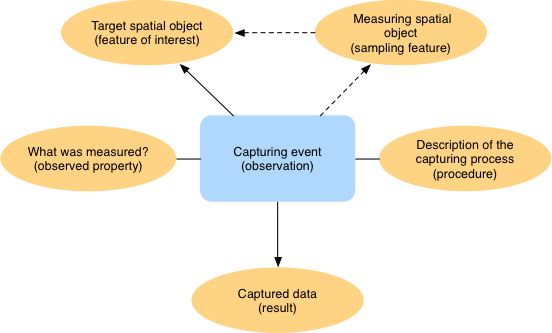
\includegraphics[]{images/basic_om_model.png}
\caption{Observations and Measurements schema}
\end{figure}

Conforming with \om\ provides a basis for extending DRS provenance concepts, by requiring that any DRS covers at least the following:
\begin{enumerate}
\item \textbf{Parties}: who is involved, ownership of the data; e.g. experimenter, institution;
\item \textbf{Procedure}: the process; e.g. model or instrument information;
\item \textbf{Sampling feature}: spatiotemporal information; e.g. the sampling frequency;
\item \textbf{Feature of Interest}:  what is measured e.g. atmosphere, ocean, clouds;
\item \textbf{Observed property}: the parameter; e.g. air temperature.
\end{enumerate}

These categories are not intended to be exclusive as there is not always a clean separation between them, particularly when one considers different perspectives.
For example, in a modelling context cloud properties may be a feature of interest but in an observational context they may be the observed property.

The procedure used for an observation (or simulation) is crucial. 
One goal of any DRS will be to provide hooks for navigation from data to information about procedures used.
Such navigation will depend on ancillary services which ideally share the same controlled vocabularies.
For example, in the case of CMIP6 the facet ``experiment" is shared by both the ESGF DRS and the Earth System Documentation system (\href{https://es-doc.org}{https://es-doc.org}), and it is possible to navigate between the DRS view of data in the ESGF and a description of the experimental protocol \citep{PasEA19} at \href{https://search.es-doc.org/?project=cmip6&documentType=cim.2.designing.NumericalExperiment&client=esdoc-url-rewrite}{es-doc.org}.

Provenance capture in a simulation workflow is relatively simple, however,
the Advanced Climate Research Infrastructure for Data \citep[ACRID, ][]{Shaon2012} project demonstrated that provenance capture is also possible for climate data observations (providing descriptions of data sources and versions, software versions, and processing options), but there is work to do do to develop appropriate linking vocabularies.
 

\section{Exploiting Data Reference Syntaxes in real systems}

The CMIP5 DRS was deployed in ESGF, as described in section \ref{s:history}. The key components of the ESGF software and workflow are shown shaded in figure \ref{cmip5-drs}: a user interface exploits a catalog and delivery services. 
The DRS provides organising principles for the catalog, and may be exploited by delivery services (including ancillary information services as discussed above).
In this section we discuss the extension of the original DRS to three important additional applications: to support the Climate Information Platform for Copernicus (CLIPC), the European Space Agency's Climate Change Indicators portal, and the sixth CMIP phase, CMIP6.

\begin{figure}
\centerline{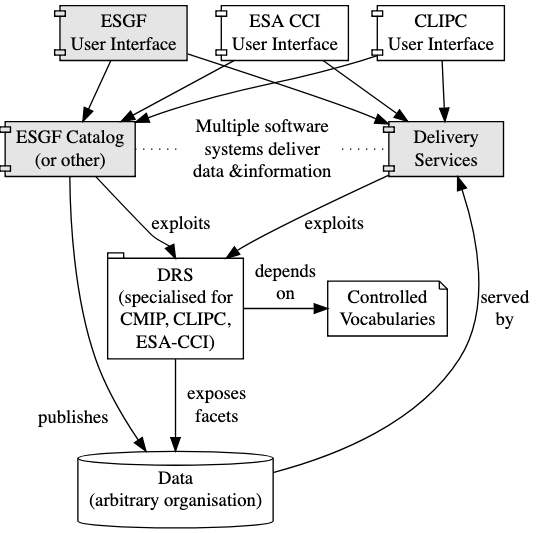
\includegraphics[width=8cm]{figs/architecture_v3.png}}
\caption{Exploiting the data reference syntax within a software system.  Data is published into catalogs, and user interfaces (discussed in the text) exploit those catalogs and a range of delivery services to allow users to navigate around data offerings before selecting and acquiring data. Such systems can exploit a Data Reference Syntax and their controlled vocabularies. \label{fig:arch}}
%TODO: Generate PDF version for final paper to increase quality
\end{figure} 

\subsection{Climate information platform for Copernicus (CLIPC)}

CLIPC \cite{} includes a heterogeneous selection of data, extending the DRS considerably from the CMIP5 usage for global modelling by including selected datasets from the Regional Downscaling Experiment (CORDEX), the Met Office Hadley Centre's HadOBS project, and climate indicators calculated from the model data.

CORDEX  was one of the first projects to be included in the ESGF as it expanded following CMIP5. It involved running regional climate models driven by boundary conditions from the CMIP5 archive for specific geographical domains \citep{Giorgi2009}. 

The CORDEX DRS \cite[described in][]{christensen2014cordex} was a relatively straightforward extension of the CMIP5 DRS, with additional terms for domain, driving model, regional climate model, and regional climate model version --- with the project facet constrained to be ``CORDEX'' (related projects with different DRS facets and project name also exist or will exist, including CORDEX-Adjust, \citealt{Nikulin2016}, and CORDEX2, \citealt{GutEA16}).
For use within the CLIPC datsets, and associated DRS, not all the CORDEX terms were required as only one 




\begin{table}[ht!]
\label{tab:cordex}
\begin{tabular}{|p{3cm}|p{9.5cm}|}
\hline
\textbf{Facet}  & \textbf{Definition}  \\ \hline
\textit{project}         & Fixed as cordex.\\ \hline
\textit{product}         & The type of output produced by the model. \\ \hline
\textit{institute}       & The institute responsible for the data.  \\ \hline
domain          & A predefined region of the global that the data covers. \\ \hline
\textit{driving model}   & The specific name of the climate model used to provide the boundary conditions. \\ \hline
experiment      & The valid CORDEX experiment short name.\\ \hline
\textit{ensemble}        & The ensemble member of the model run, inherited from the global model run; given in the form r\textless{}L\textgreater{}i\textless{}M\textgreater{}p\textless{}N\textgreater where, L M and N are integers and r is for realisation; i for initialisation and p is for physics. \\ \hline
rcm\_name        & The regional climate model name.    \\ \hline
rcm\_version     & The regional climate model version.    \\ \hline
\textit{time frequency}  & The temporal frequency of the output data. \\ \hline
\textit{variable}        & The short variable name identifier. \\ \hline
\textit{version}         & This is an ESGF version to uniquely identify the dataset and version control the data, it is given the form vYYYYMMDD. \\
\hline

\end{tabular}
\caption{Facet definitions for CORDEX. Facets denoted with italics share the same controlled vocabulary as used for CMIP5, except for driving model, where that facet  uses the CMIP5 source facet vocabulary.
These facets are connected together using a ``." to construct the unique DRS: 
\textless{}project\textgreater{}.\textless{}product\textgreater{}.\textless{}domain\textgreater{}.\textless{}institute\textgreater{}.\textless{}driving\_model\textgreater{}.\textless{}experiment\textgreater{}.\textless{}ensemble\textgreater{}.\newline\textless{}rcm\_name\textgreater{}.\textless{}rcm\_version\textgreater{}.\textless{}time\_frequency\textgreater{}.\textless{}variable\textgreater{}.\textless{}version\textgreater{}
 \label{t:cordex}}
\end{table}


A CMIP5 DRS example is \newline 
\small{\texttt{cordex.output.AFR-44.DMI.ECMWF-ERAINT.evaluation.r1i1p1.HIRHAM5.v2.day.uas.v20140804}}

The CORDEX data is hosted directly by the ESGF, with a subset indexed within CLIPC. The necessary DRS to work with the ESGF was established as a fairly direct extension from CMIP5 (table \ref{t:cordex}), and is subsumed directly into CLIP-C.
The more widely used DRS elements that were are required for the publication of model data were not always appropriate for observational data

In this section four different project DRS are considered; they are the CMIP5, Regional Downscaling Experiment (CORDEX), ESA Climate Change Initiative (CCI) and the Met Office Hadley Centre (MOHC) HadOBS projects. The CMIP5 project is a modelling project, CORDEX is a regional modelling project, the ESA-CCI project is an satellite observation project and the HadOBS project is a ground based observations project.  


Table \ref{tab:drs-schema} shows the DRS elements used in each of the projects CMIP5, CORDEX, ESA-CCI and HadOBS respectively. The facets shown in normal font are unique facets for a given project the facets in grey italics are facets already defined and can be utilised by multiple projects. Since CMIP5 was the first project to use this approach to data discovery all the facets used were uniquely defined for this project. 

These facets are connected together using a ``." to construct the unique DRS: 
\textless{}project\textgreater{}.\textless{}product\textgreater{}.\textless{}domain\textgreater{}.\textless{}institute\textgreater{}.\textless{}driving\_model\textgreater{}.\textless{}experiment\textgreater{}.\textless{}ensemble\textgreater{}.\newline\textless{}rcm\_name\textgreater{}.\textless{}rcm\_version\textgreater{}.\textless{}time\_frequency\textgreater{}.\textless{}variable\textgreater{}.\textless{}version\textgreater{}
A CMIP5 DRS example is \newline 
\small{\texttt{cordex.output.AFR-44.DMI.ECMWF-ERAINT.evaluation.r1i1p1.HIRHAM5.v2.day.uas.v20140804}}.
\normalsize

\subsubsection{ESA-CCI: ESA Climate Change Initiative}
The European Space Agency Climate Change Initiative (ESA-CCI) project is the first remotely sensed data to be published in ESGF and it required a number of new facets. Firstly consider the provenance facets. The term project is introduced and it is now common place to use project rather than activity and they are often used interchangeably. The product facet in the modelling community has a different meaning to that used in the EO community, therefore to work with the existing infrastructure the facet ``product string" was included, where ``product string" is the typical name of the EO product. The observation community also commonly have product versions associated with their data to keep up-to-date with the most recent observations and methodologies this was not required in the CMIP program and so an additional facet was introduced to describe this.  There are also a number of additional procedural facets that are required to describe the ESA-CCI data, they are the processing level, sensor id and platform id. 

\begin{table}[ht!]
\label{tab:cci}
\begin{tabular}{|p{3cm}|p{9.5cm}|}
\hline
\textbf{Facet}  & \textbf{Definition}  \\ \hline
project         & Fixed as clipc\\ \hline
product         & The type of output; esacci \\ \hline
cci project     & The ESA CCI essential climate variable project. \\ \hline
time frequency  & The temporal frequency of the output data.  \\ \hline
processing level    & The level of processing applied to the observational data, e.g. L3, L4.  \\ \hline
CCI geophysical parameter  & The observed quantity.  \\ \hline
sensor          & The instrument name. \\ \hline
platform        & The satellite that carried the sensor.    \\ \hline
product string  & An additional product descriptor required for uniqueness, could be the name of a processing algorithm. \\ \hline
product\_version & A version commonly associated with the dataset. \\
realization     & The ensemble member. \\ \hline
version         & This is an ESGF version to uniquely identify the dataset and version control the data, it is given the form vYYYYMMDD. \\
\hline

\end{tabular}
\caption{Facet definitions for ESA CCI}
\end{table}
The CCI facets were connected together to produce unique dataset identifiers of the form:

\noindent\textless{}project\textgreater{}.\textless{}cci\_project\textgreater{}.\textless{}time\_frequency\textgreater{}.\textless{}processing\_level\textgreater{}.\textless{}cci\_geophysical\_parameter\textgreater{}.\\\textless{}sensor\_id\textgreater{}.\textless{}platform\_id\textgreater{}.\textless{}product\_string\textgreater{}.\textless{}product\_version\textgreater{}.\textless{}realization\textgreater{}.\textless{}esgf\_version\textgreater{}

A CMIP5 DRS example is \newline
\small{\texttt{{clipc.esacci.CLOUD.day.L3U.CLD\_PRODUCTS.MODIS.Aqua.MODIS\_AQUA.1-0.r1.v20120704}}.\normalsize


\subsubsection{MOHC HadOBS: Met Office Hadley Centre, observational data products}
The MOHC HadOBS observational data also required additional provenance information to describe the data effectively.

\begin{table}[ht!]
\label{tab:hadobs}
\begin{tabular}{|p{3cm}|p{9.5cm}|}
\hline
\textbf{Facet}  & \textbf{Definition}  \\ \hline
project         & Fixed as CLIPC\\ \hline
product         & The type of data \\ \hline
institute       & The institute responsible for the data. \\ \hline
framework       & Dataset framework  \\ \hline
collection      & The dataset collection \\ \hline
frequency       & The temporal frequency of the output data.  \\ \hline
realization     & The ensemble member. \\ \hline
product\_version & A version commonly associated with the dataset. \\ \hline
version         & This is an ESGF version to uniquely identify the dataset and version control the data, it is given the form vYYYYMMDD. \\
\hline

\end{tabular}
\caption{Facet definitions for HadOBS}
\end{table}

These facets are connected together using a ``." to construct the unique DRS: 
\noindent\textless{}project\textgreater{}.\textless{}product\textgreater{}.\textless{}institute\textgreater{}.\textless{}framework\textgreater{}.\textless{}collection\textgreater{}.\textless{}frequency\textgreater{}.\\\textless{}realization\textgreater{}.\textless{}product\_version\textgreater{}.\textless{}esgf\_version\textgreater{}
A CMIP5 DRS example is \newline 
\small{\texttt{clipc.insitu.MOHC.HadOBS.HadISDH.mon.r1.v2-1-0-2015p.v20151231}}.\normalsize

\begin{figure}[ht!] \label{fig:clipc-hadobs}
\centering
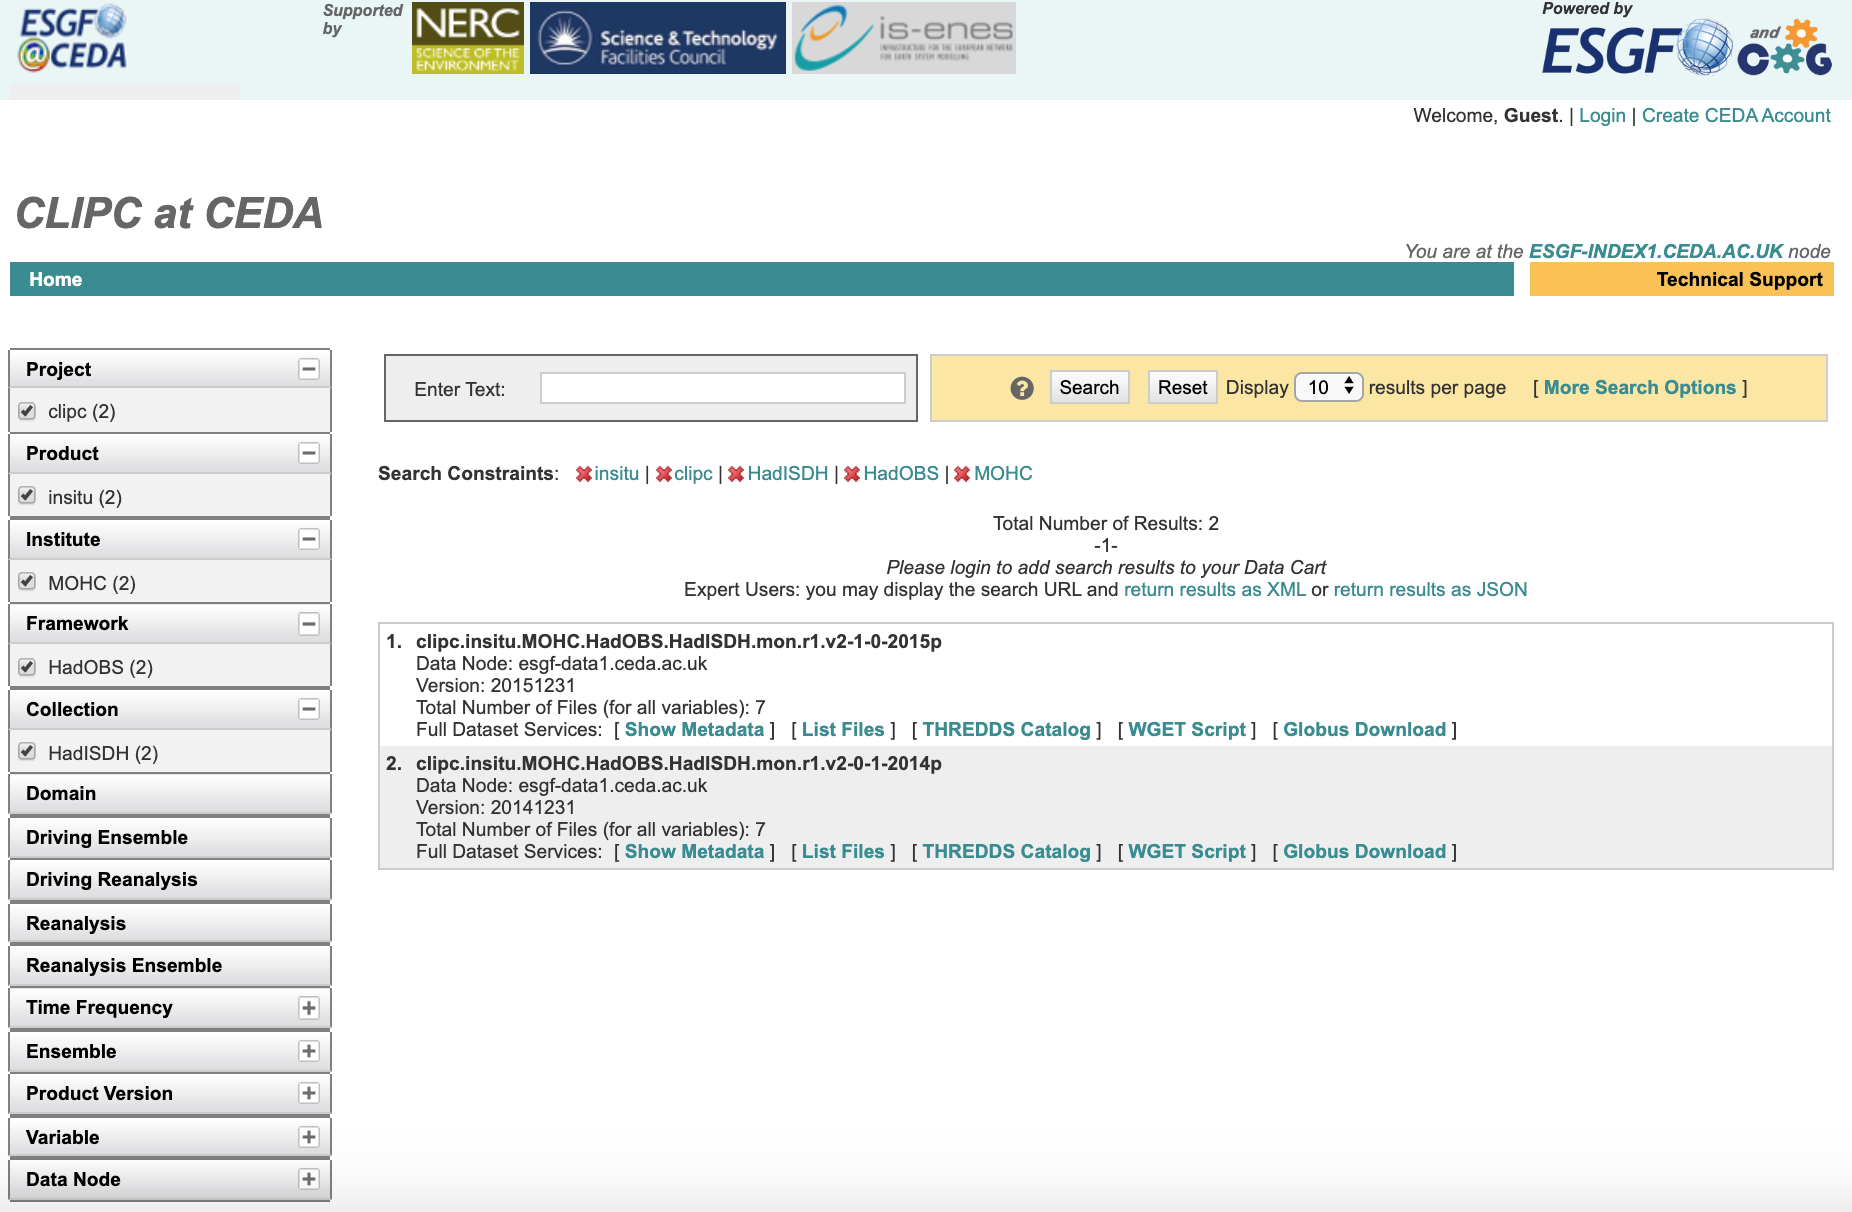
\includegraphics[scale=0.4]{images/clipc-esgf-search.png}
\caption{Example ESGF search for insitu observational data}
\end{figure}

\subsection{CMIP6}
Although not a part of the CLIPC project, since that project took place the phase 6 CMIP data (CMIP6) is now being released and the DRS have been defined as shown it the table \ref{tab:cmip6}. Many similar facets are common between CMIP5 and CMIP6 however some have been renamed ** this is not good practice why oh why **. The largest change from CMIP5 to CMIP6 is the granularity level of the DRS. In CMIP5 all variables for a given dataset were included within the dataset. There were often many 20-30 variables within a dataset. This was not optimal from a search or data management perspective. Therefore within CMIP6 the variable has been elevated to be a distinct facet. This is extremely useful given the much larger volume of CMIP6. For example a user may simply be interested in a couple of variables for example sea ice and sea surface temperature, a user can simply search for these two variables and then narrow down their search from there. 

\begin{table}[ht!]
\label{tab:cmip6}
\begin{tabular}{|p{3cm}|p{9.5cm}|}
\hline
\textbf{Facet}  & \textbf{Definition}  \\ \hline
mip\_era         & The phase of CMIP in this case CMIP6; equivalent to the CMIP5 project.\\ \hline
activity\_drs    & The model intercomparison project (MIP) to which the data belong. \\ \hline
institution\_id  & The climate modelling centre(s) or University responsible for the model. \\ \hline
source\_id       & The specific name of the climate model used.  \\ \hline
experiment\_id   & The valid CMIP6 experiment short identifier.  \\ \hline
member\_id       & The specific ensemble member of the model run of the form r\textless{}L\textgreater{}i\textless{}N\textgreater{}p\textless{}M\textgreater{}f\textless{}R\textgreater where, L, M, N and R integers and r is for realisation; i for initialisation; p is for physics and f is for forcing. \\ \hline
table\_id        & A lookup table that relates the frequency of a variable and its realm. \\ \hline
variable\_id     & A short variable name identifier. \\ \hline
grid\_label      & A short grid type identifier. \\ \hline
Version         & This is an ESGF version to uniquely identify the dataset and version control the data, it is given the form vYYYYMMDD. \\
\hline

\end{tabular}
\caption{Facet definitions for CMIP6}
\end{table}

These facets are connected together using a ``." to construct the unique DRS: 
\textless{}mip\_era\textgreater{}.\textless{}activity\_drs\textgreater{}.\textless{}institution\_id\textgreater{}.\textless{}source\_id\textgreater{}.\textless{}experiment\_id\textgreater{}.\textless{}member\_id\textgreater{}.\newline\textless{}table\_id\textgreater{}.\textless{}variable\_id\textgreater{}.\textless{}grid\_label\textgreater{}.\textless{}version\textgreater{}

A CMIP6 DRS example is \newline \small{\texttt{CMIP6.CMIP.AWI.AWI-CM-1-1-MR.historical.r5i1p1f1.3hr.rldscs.gn.v20181218}.\normalsize

\subsection{Analysis of DRS extensions}


\begin{table}[htb!]
\label{tab:drs-schema}
\small
\begin{tabular}{p{1.4cm} p{2.0cm} p{2.1cm} p{2.1cm} p{1.4cm} p{2.0cm} }
	& \textbf{Provenance} & \textbf{Procedure} & \textbf{Sampling} & \textbf{Feature} & \textbf{Parameter} \\[2pt]  \hline 
 \\      
\textbf{CMIP5} & activity & model & frequency & realm & variable name \\ 
	& product & experiment &  & cmor\_table & \    \\ 
	& institute & ensemble & \  & \  & \   \\[2pt]   \hline 
\\[-4pt]      
\textbf{CORDEX} &  {\textit{activity}} & domain &  {\textit{frequency}}   & \  & \    \\ 
                &  {\textit{product}}  & driving\_model  & \  & \  & \    \\ 
                &  {\textit{institute}} & experiment  & \  & \  & \    \\ 
                & &  	 {\textit{ensemble}}   & \  & \  & \    \\ 
                & & 	 {\textit{model}}    & \  & \  & \  \\ 
                & & 	rcm\_version     & \  & \  & \  \\[2pt] 
   \textbf{HadOBS} & framework & \  & \  & \   \\[2pt]
 & 	collection & \  & \  & \  & \    \\[2pt] 
\textbf{ESA-CCI} &  project & processing level & time\_frequency & cci\_project & cci\_geo\_quantity$^*$  \\ 
& 	product\_string & sensor id & \  & \  & \  \\ 
& 	product\_version & platform id & \  & \  & \   \\ 
\ & \ & realization & \ & \ & \\[2pt]  \hline
 \\[-4pt]
 \textbf{CMIP6} & mip\_era & source\_id & nom\_resolution$^*$ & realm& variable \\
  & activity & experiment\_id & sub-experiment & table id  & cf\_std \_name$*$ \\
  & model\_cohort & source\_type & grid label &  \\
  & product &  variant\_label & frequency & \\
  & institution\_id &  & & \\[2pt] \hline

\end{tabular}
\caption{DRS elements classified by schema element. (terms with $^*$ suffix have been abbreviated for presentation)}
%TODO: Expand table caption, move to later
\end{table}




\section{Improving navigability}

The benefit of using controlled vocabularies include flexibility, scalability and the linking of information subsystems. 

One example of a mature controlled vocabulary within the Climate Science community is the Climate and Forecast (CF) standard names ?REF?. This is a list of variables names used in the climate and forecast community. Each term has precise spelling and definition. For example,  air\_pressure\_at\_sea\_level has the definition ``sea\_level means mean sea level, which is close to the geoid in sea areas. It is defined as having canonical units of Pascals (Pa).  Having precise definitions means that meteorologists and climate scientists anywhere in the world using this standard name know that they are referring to the same quantity. This becomes ever more important when considering more complex variables for example radiative fluxes which have a vector component of direction and can be absolute or net. Having a name which clearly specifies the direction of the radiation and whether it is the absolute or net value is vital to ensure that variables are compared correctly or radiative budgets calculated correctly.     

Using CVs is an essential component of a DRS, however CVs must be managed and the complexity of these can vary. In the simple example of the ``realm" facet of CMIP5 there are only seven terms in the CV. Where there are only a small number of terms they could be managed for example in GitHub like many of the controlled vocabularies for CMIP6 as they require minimal management. In contrast the CF standard name table (a CV) currently consists of around 6000 terms and is managed by community experts. In order to add a new standard name to the table, it must be proposed, moderated (by the community experts) and approved; this involves a substantial amount of effort and collaboration. It is recommended that when using a CV in a DRS where possible the terms should be taken from existing CVs. In comparing the terms used in the ``frequency" facet it has been noticed that different data producers sometimes use subtly different terminology. For example, it is not uncommon to see year and yr, or monthly and mon. While it is possible to use semantic web technologies such as SKOS to relate these terms it is most beneficial if terms were used consistently. 

% Within the CMIP5 and CMIP6 projects, which are large international collaborations specialist documentation and distribution software has been used and is in development, these projects have necessarily had to develop and utilise large CVs.

A number of new controlled vocabularies have been defined for CLIPC. The content of these new controlled vocabularies has been defined in consultation with the data providers and curators. Provenance information is currently represented using PROV-O for new vocabularies to be incorporated into the NERC Vocabulary Server (NVS). The new vocabularies for CLIPC included defining conceptual schemes or themes such as the Global Climate Observing System (GCOS) Essential Climate Variable (ECV) domains and subdomains: atmospheric, terrestrial, atmospheric surface, atmospheric upper-air, atmospheric composition, oceanic surface, oceanic sub-surface. To reconcile the different vocabularies for the different climate data records the Simple Knowledge Organisation System (SKOS) is used to provide a mapping framework that links terms from different vocabularies using semantic mappings. 

SKOS provides relational matches between two predefined vocabularies using the Resource Description Framework (RDF). The SKOS relationships between different vocabularies can be loosely defined as 

\begin{itemize}
    \item associative: concepts are related, they may be approximately interchangeable; can be either close or exact relationships
    \item hierarchical: concepts can be broader or narrower:
        \begin{itemize}
            \item broader: the current term has a more specific definition than the related term e.g. carbon dioxide has a broader relationship to greenhouse gases
            \item narrower: the current term has a less specific definition than the related term e.g. atmospheric composition has a narrower relationship to greenhouse gases
        \end{itemize}
\end{itemize}

Using SKOS the internal hierarchical and associative mappings are defined, this allows terms within and across different controlled vocabularies to be related greatly enriching the data search experience. 

\subsection{The Climate Change Initiative (CCI) example}

The data reference syntax that were defined in \ref{tab:cci} for the ESA CCI project were used not only in the CLIPC project but also in the ESA CCI portal. 
Here a faceted search was implemented on the data utilising the linked data technologies to enhance search and discovery. 
Example:

Screenshot:




%TODO: Lessons learned: CORDEX wild west, CMIP changing facets. Trade off between ease of use for producers and consumers.





\section{Summary and Future Work}

The first use of DRS in the CMIP5 project provided a comprehensive list of facets that were relatively simply managed. A DRS:

\begin{itemize}
\item provides a unique identifier for the dataset,
\item provides a common terminology for a collection of datasets,
\item can aid filesystem management,
\item allows faceted searching.
\end{itemize}

Since then many new projects have emerged that use the ESGF infrastructure for publication and thus need a good DRS in order to provide a good quality faceted data search. A number of problems are now emerging and they are detailed below. 

There must be robust communication in this multi-disciplinary environment as this is a community exercise with technical constraints. 

\subsection{Lessons learned}
\subsection{Governance}
- The importance of maintenance of information . . . facet name inconsistencies eg table, table\_id 
- Difficulties of a globally distributed differential funded environment on information management. Having all the controlled vocabularies for each project stored in a central GitHub repository - even this has its problems...
- social concept of communications costs necessary ... link to the vocabularies as being key to this.
\subsection{Flexibility and Futures}


\section*{SOME FIGURES}

The CLIPC portal allows users access to a visualisation tool 



\begin{figure}
    \centering
    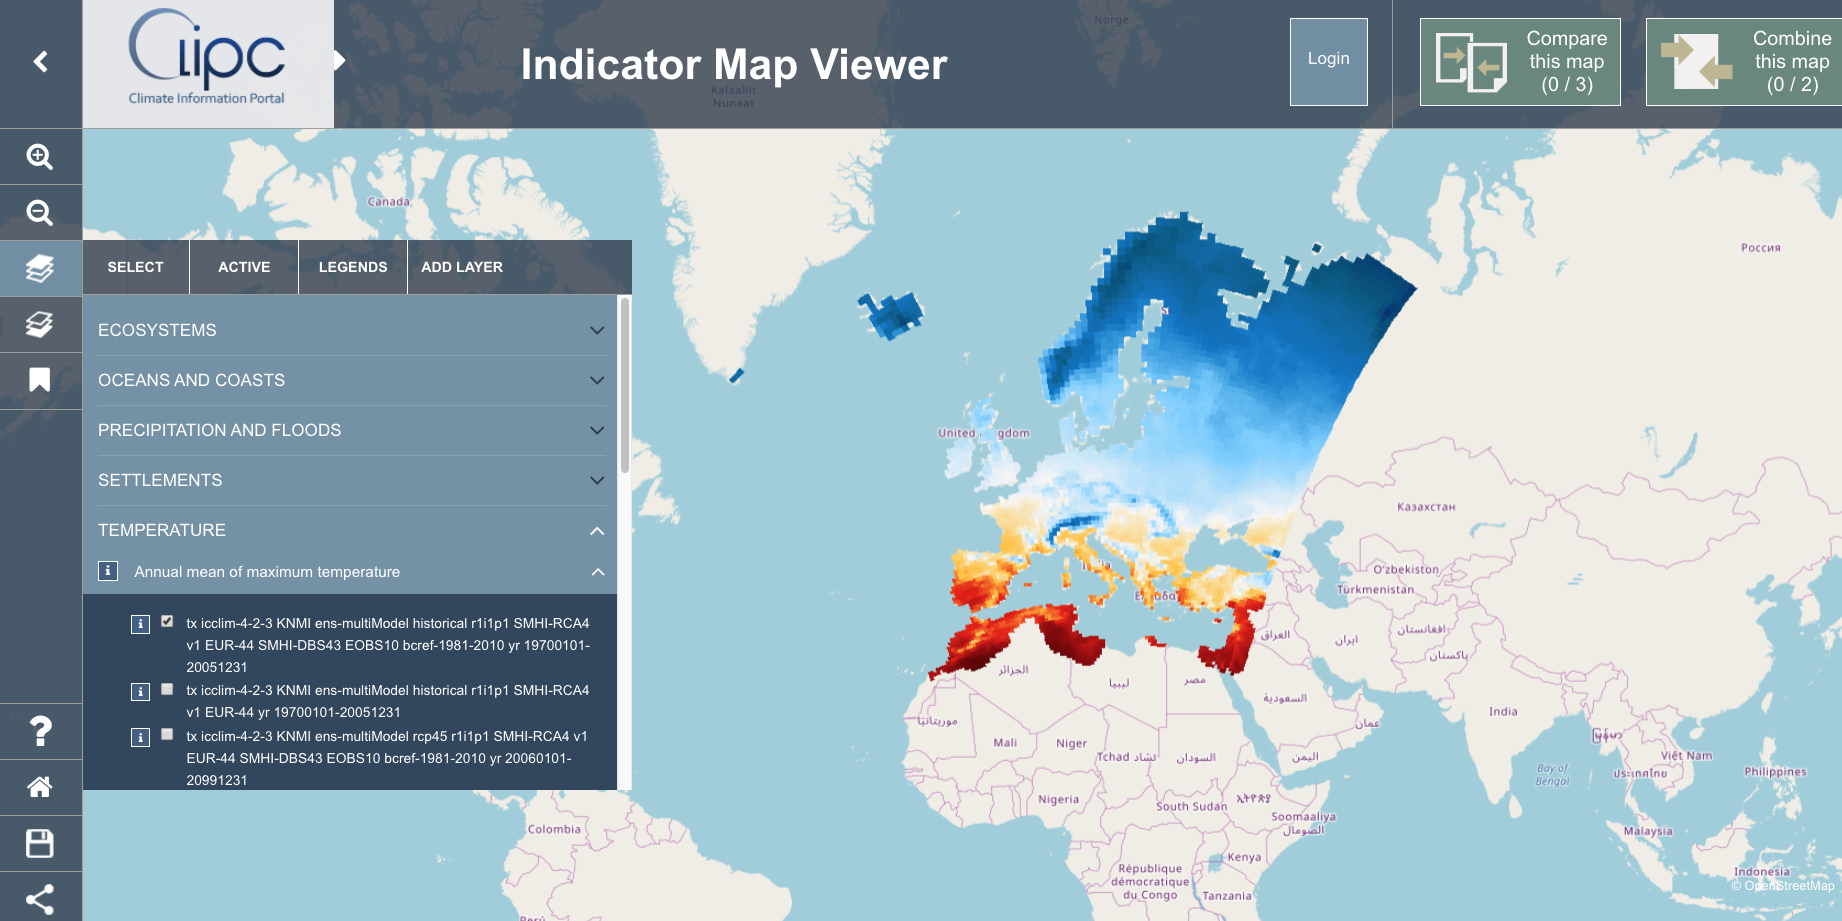
\includegraphics[scale=0.2]{images/c4iportal.png}
    \caption{Mapping tool from CLIPC toolbox (If we use ths one will need to in introduce the DRS for the impact indicators)}
    \label{fig:my_label}
\end{figure}


Main CLIPC SEARCH
\begin{figure}
    \centering
    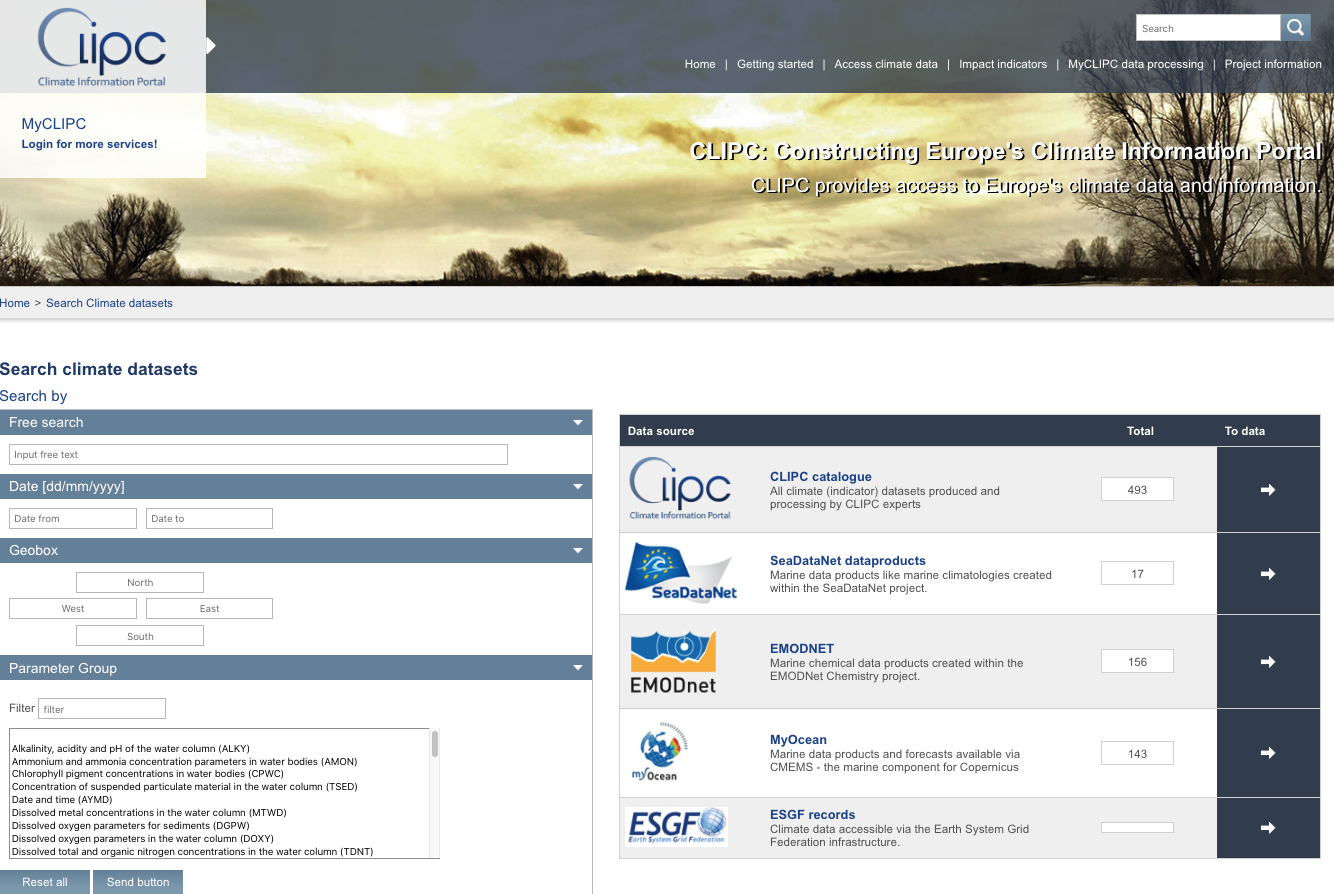
\includegraphics[scale=0.3]{images/CLIPC-seach.png}
    \caption{CLIPC data search}
    \label{fig:my_label}
\end{figure}


CLIPC as found in C4I
\begin{figure}
    \centering
    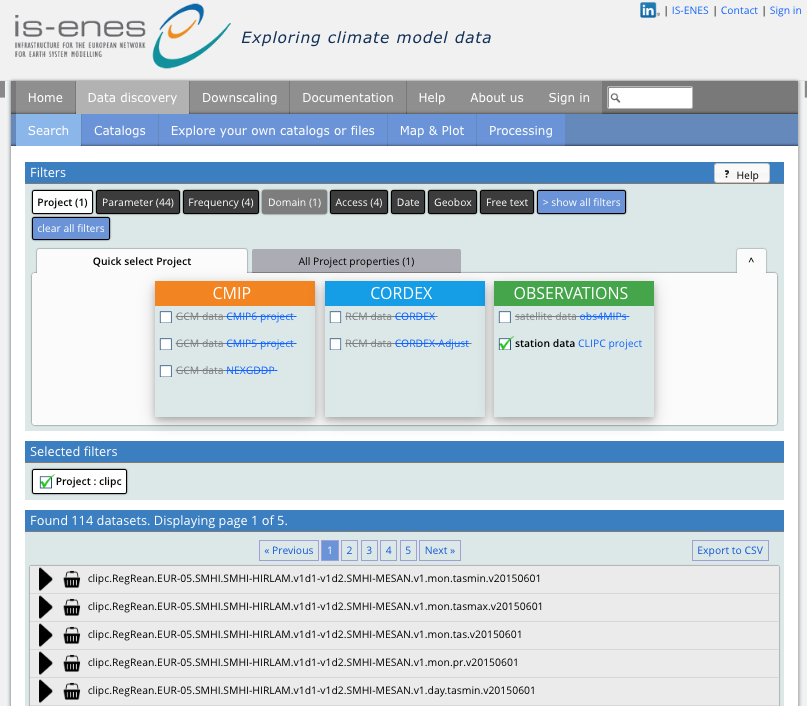
\includegraphics[scale=0.4]{images/CLIPC-search-in-C4I.png}
    \caption{CLIPC data search through Climate for impacts portal}
    \label{fig:my_label}
\end{figure}



CCI 
\begin{figure}
    \centering
    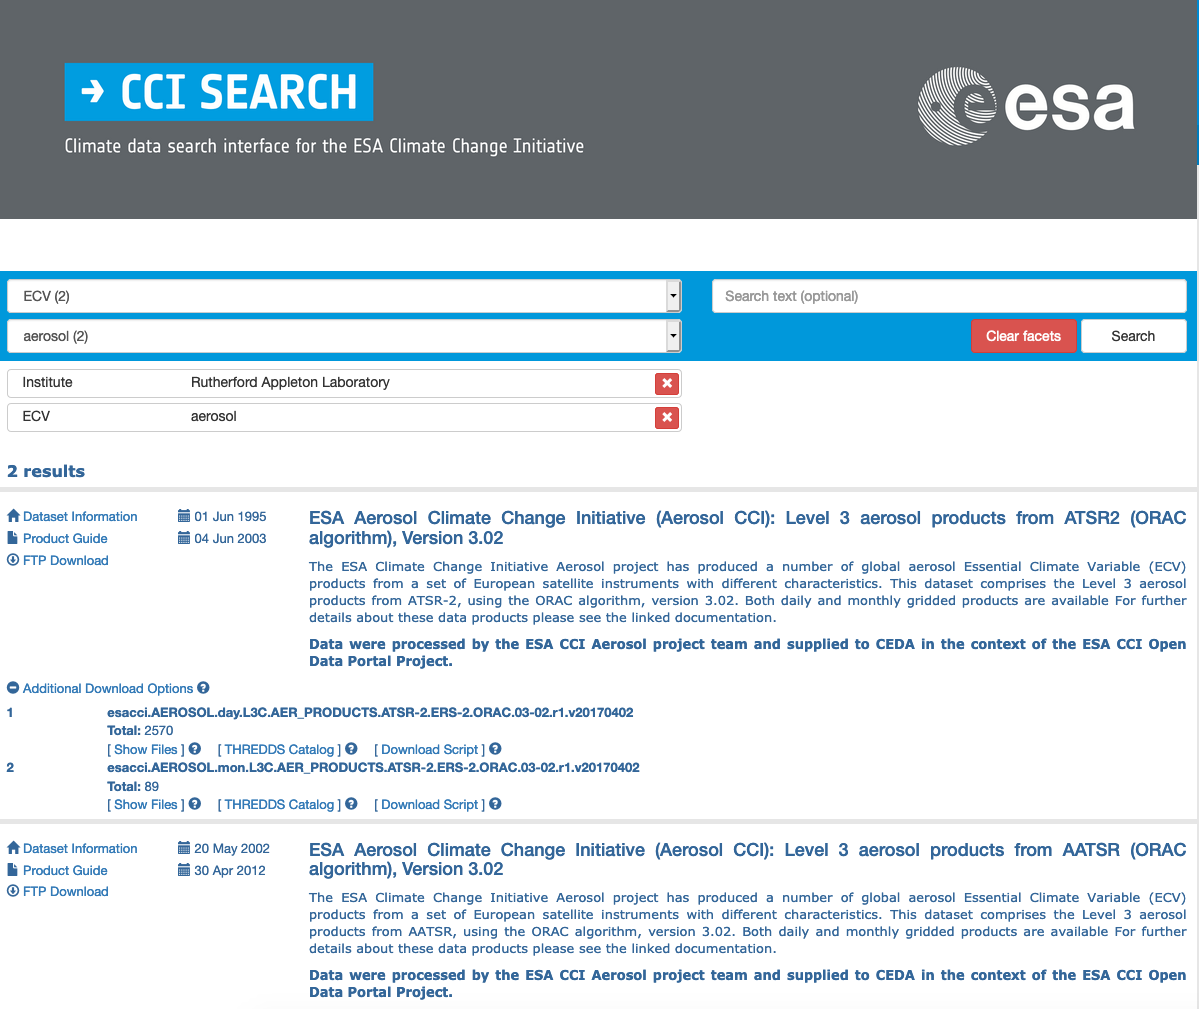
\includegraphics[scale=0.3]{images/CCI.png}
    \caption{CCI}
    \label{fig:my_label}
\end{figure}


%% The Appendices part is started with the command \appendix;
%% appendix sections are then done as normal sections
%% \appendix

%% \section{}
%% \label{}

%% If you have bibdatabase file and want bibtex to generate the
%% bibitems, please use
%%
\bibliographystyle{elsarticle-harv} 
\bibliography{biblio}

%% else use the following coding to input the bibitems directly in the
%% TeX file.

% \begin{thebibliography}{00}

% %% \bibitem[Author(year)]{label}
% %% Text of bibliographic item

% \bibitem[ ()]{}

% \end{thebibliography}

% \newpage
% \appendix \label{App:1}
% \LARGE\textbf{Appendix I: Facet definitions for projects within this paper}
% \normalsize
% \begin{longtable}{  p{1.8cm} | p{4.2cm} | p{5cm} | p{1.1cm} | p{3cm}  }
% \hline
% 	\textbf{Project} & \textbf{Facet} & \textbf{Definition} & \textbf{Format} & \textbf{Value Example} \\ \hline
% 	\textbf{CMIP5} &  &  &  &  \\ \hline
% 	 & activity & Model intercomparison activity or other data collection activity & CV & cmip5 \\ \hline
% 	 & product & Type of CMIP output & CV & output1 \\ \hline
% 	 & institute & Institute responsible for the model results & CV & MPI-M \\ \hline
% 	 & model & Model used and its version & SF & MPI-ESM-LR \\ \hline
% 	 & experiment & identifies either the experiment or both the experiment family & CV & abrupt4xCO2 \\ \hline
% 	 & Frequency & Temporal frequency of output & CV & mon \\ \hline
% 	 & modelling realm & High level modeling component  & CV & atmos \\ \hline
% 	 & MIP table & MIP reference lookup table for variable name & CV & Amon \\ \hline
% 	 & ensemble member & Ensemble member reference code & SF & r1i1p1 \\ \hline
% 	 & version number & Dataset publication version as date  & SF & v20120602 \\ \hline
% 	 & variable name & Abbreviation of variable name given by MIP table & CV & --many-- \\ \hline
% 	\textbf{CORDEX} &  &  &  &  \\ \hline
% 	 & activity & Name of project & Fixed & cordex \\ \hline
% 	 & product & Type of output & Fixed & output \\ \hline
% 	 & domain & CORDEX domain name & CV & EUR-44 \\ \hline
% 	 & institution & Acronym of the institution responsible for the simulation & CV & MOHC \\ \hline
% 	 & GCMModelName & Driving model name or reanalysis data used as the driving data  & CV & ECMWF-ERAINT \\ \hline
% 	 & CMIP5ExperimentName & Driving experiment name, evaluation or CMIP5 experiment\_id & CV & evaluation \\ \hline
% 	 & CMIP5EnsembleMember & Driving model ensemble member  & SF & r0i0p0 \\ \hline
% 	 & RCMModelName & Regional Climate Model name identifier (<instiution>-<regional model>) & CV & MOHC-HadGEM3-RA  \\ \hline
% 	 & RCMVersionID & Regional Climate Model version identifier  & Free string & v1 \\ \hline
% 	 & Frequency & Temporal frequency of output & CV & 3hr \\ \hline
% 	 & variable name & CMIP5 variable name abbreviation & CV & clt \\ \hline
% 	 & version number & Dataset publication version as date  & SF & v20120602 \\ \hline
% 	 &  &  &  &  \\ \hline
% 	\textbf{CCI} &  &  &  &  \\ \hline
% 	 & project & Project name & Fixed & clipc \\ \hline
% 	 & product & product type & Fixed & esacci \\ \hline
% 	 & cci\_project & The ESA CCI Essential Climate Variable project & CV & CLOUD \\ \hline
% 	 & time\_frequency & Temporal frequency of output, yr, mon, day, etc & CV & day \\ \hline
% 	 & processing\_level & The processing level of the data, e.g. L3, L4 & CV & L3U \\ \hline
% 	 & data\_type & The parameter assessed & CV & CLD\_PRODUCTS \\ \hline
% 	 & sensor\_id & The remote sensing instrument name & CV & MODIS \\ \hline
% 	 & platform\_id & The satellite platform that the sensor instrument is on & CV & Aqua \\ \hline
% 	 & product\_string & Product name, sometimes an algorithm & SF & MODIS\_AQUA \\ \hline
% 	 & product\_version & product version number & SF & 1-0 \\ \hline
% 	 & realization & ensemble version & SF & r1 \\ \hline
% 	 & version number & Dataset publication version as date  & SF & v20120704 \\ \hline
% 	 &  &  &  &  \\ \hline
% 	\textbf{HadOBS} &  &  &  &  \\ \hline
% 	 & project & CLIPC & Fixed & clipc \\ \hline
% 	 & product & Type of product & CV & insitu \\ \hline
% 	 & inst & Institute & CV & MOHC \\ \hline
% 	 & framework & Dataset framework & CV & HadOBS \\ \hline
% 	 & collection & Name of data product & CV & HadISD \\ \hline
% 	 & frequency & Temporal frequency of output & CV & subdaily \\ \hline
% 	 & table & ? include - not been needed? &  &  \\ \hline
% 	 & realization & Ensemble member & SF & r1 \\ \hline
% 	 & product\_version & Product version number & SF & 1-0-4-2015p \\ \hline
% 	 & version & Dataset publication version as date  & SF & v20151231 \\ \hline
% \end{longtable}

\end{document}

\endinput
%%
%% End of file `elsarticle-template-harv.tex'.
